%----------------------------------------
% Preamble to set up the document
%----------------------------------------
\documentclass{article}

% set up packages (you shouldn't need to touch this)
\usepackage{graphicx}  % required to insert images
\usepackage{hyperref}  % for hyperlinks
\usepackage[svgnames]{xcolor}  % to change hyperlink colors
\colorlet{linkcolour}{DarkBlue}
\hypersetup{colorlinks=true, linkcolor=linkcolour, citecolor=linkcolour, urlcolor=linkcolour,}

% Margins
\topmargin=-0.45in
\evensidemargin=0in
\oddsidemargin=0in
\textwidth=6.5in
\textheight=9.0in
\headsep=0.25in

% use a sans serif font
\renewcommand{\familydefault}{\sfdefault}

%----------------------------------------
% Step 1: Edit the lecture title
%----------------------------------------
\title{
Lecture 5: Reproducibility, replication, etc \\  % Lecture title
Modeling Social Data, Spring 2019 \\   % Course title
Columbia University                    % School
}

%----------------------------------------
% Step 2: Edit your name and the date
%----------------------------------------
\author{Sagar Lal}                     % Scribe's name
\date{February 22, 2019}                % Lecture date

\begin{document}

\maketitle


%----------------------------------------
% Step 3:
% Rename uni.tex to match your uni,
% edit the filename accordingly below,
% and put your notes in this file
%----------------------------------------
%----------------------------------------
% Write your notes here
%----------------------------------------

\section{Introduction}
\subsection{Motivation for the lecture:}
\begin{itemize}
    \item{Currently,we are seeing lots of issues with reproducibility and replication in Social Science academia, as well as in astronomy and the life sciences.}
    
    \item{This seems to happen because professors would get tenure from shiny results, so they occasionally had dubious approaches to achieve these results.}
    
     \item {Up until now we (students) have only been “producing” results, now we are going to look at analyzing/critiquing results to hopefully get rid of bad science and only get good scientific papers published.}

\end{itemize} 

\subsection{Key Questions to consider in evaluation research:}

\begin{itemize}
    \item{Was the research done and reported honestly/correctly?}
    
    \item{Is the result "real" or an artifact of the data?}
    
    \item {Will it hold up over time?}
    
    \item {How robust is the result to small changes?}
 
    \item {How important/useful is the finding?\\}

\end{itemize} 

\section{Honesty}
\textbf{Was the data reported and collected honestly:} 
We’ll take the optimistic view point that most researches are honest, and mistakes are due to stupidity, but that is not always the case.

\subsection{ \textit{When Contact Changes Minds}: A Social Science Example of honesty failing}
\subsubsection{The experiment}
\begin{itemize}
    \item{Ask question: Can a single conversation change people’s belief on gay marriage}
    
    \item{Someone knocks on your door to talk to you about talking gay rights (might present yourself as straight/gay whether you are or not)}
    
    \item {This conversation changes your view in the moment. Furthermore if the person who knocked on the door said they were gay, the results were more persistent}
    
    \item The idea was that this meant that more people could knock on doors to shift public perception
    
\end{itemize}

\subsubsection{Questioning of Results and Reproducibility}
\begin{itemize}
    \item{Irregularities in LaCour (2014) showed that the results were pretty dubious}
    
    \item Looked at public opinion polls that were so different from the paper’s results
    
    \item But they thought question was interesting so they went to analyze it with transgender

    \item {Found that conversations decreased transphobia at a greater rate and that the results persisted for 3 months, regardless if canvasser was trans or not.\\}
    
\end{itemize}
\section{Reproducibility}
\textbf{Can you independently verify the exact results using the same data and the same analysis}

\subsection{Though a low bar, most research doesn’t currently pass this test}

\begin{itemize}
    \item{Data or code aren’t available/complete}
    
    \item Code is difficult to run/understand
    
    \item Complex software dependencies
    
    \item Full reproducibility is not part of the current pipeline. Due to dependencies or code being complex even if it’s given to you it’s tough run
    
\end{itemize}

\subsection{This is improving with better software engineering practices among researchers}

\begin{itemize}
    \item{Literate programming (Jupyter, Rmarkdown)}
    
    \item Automated build scripts (Makefiles) 
    
    \item Containers (Docker, Code Ocean)
    
    \item Currently, the ACM (association for computing machinery which is main CS society) puts badges on papers if example code is provided and is functional to use.
    
\end{itemize}

\subsection{Practical Constraints that make this not a hard rule}

\begin{itemize}
    \item{\href{https://blog.openai.com/better-language-models/}{Open AI last week published} a better language model that can be misused so they only published a fraction of their research.}
    
    \item For example: Private company wants to publish paper that used a 50k GPU etc, doesn’t want to give out their own private repository and not everyone has access to this GPU
    
    \item Jake can’t publish the Twitter data that he worked with due to privacy concerns as well as general data access decision by Twitter 
    
    \item \href{https://openreview.net/pdf?id=B1eYYK5QgX}{A practical taxonomy of reproducibility for ML research} is a paper from 2018 by UW professor and Kaggle team. They analyzed the NIPS conference (where 6k submissions only 700 accepted) only 40\% of accepted papers provided links to work
    
\end{itemize}

\section{Replicability}

\subsection{Will the result hold up with new data but the same analysis?}

\begin{itemize}
    \item It’s easy to be fooled by randomness
    
    \begin{itemize}
        \item For example seeing that sending people to the door to talk about gay rights changes people’s opinions. 
        \item You get results and it seems that there is an effect, but not persist because you’re just looking at noise. 
        \item Small datasets of size of 50 are common in political science, which can make it especially difficult to draw conclusions
    \end{itemize}

    \item Noise can dominate signal in small datasets
    
    \item Asking too many questions of the data can lead to overfitting
    
    \begin{itemize}
        \item For example you keep y the same, but you add more and more x’s to see how they impact y and eventually find a perfectly predictive model but it might not hold up 
        \item Tangential relationship to bias-variance trade off
        \item \href{https://xkcd.com/1122/}{XKCD election replicability comic}
    \end{itemize}
\end{itemize}
\subsection{Replicability Crisis Example}
\begin{itemize}
    \item People at open science in Virginia (Brian Nozick) wanted to redo 100 different psych experiments to check to see if the results were replicable. They conducted 100 psych experiments 
    \item Results
    \begin{itemize}
        \item Replication effects were half the magnitude of original effects
        \item 97\% of original studies had statistically significant results, while in this study 36\% of replicated studies had statistically significant results
        \item Only 47\% of original results were within the 95\% confidence interval
        \item The effect size versus replication shows how the independent variable effect size was rarely as strong as stated. In fact some times the effect size was negative when reported positive. 
        \begin{itemize}
            \item Effect size indicates the difference in mean of two distributions, ie the impact of a drug on health compared to that of placebo on health
        \end{itemize}
    \end{itemize}
    \item There is a clear crisis going on that suggests that you should basically believe about half of what you read for some scientific journals
    \begin{itemize}
        \item Jake believes it’s more bad science rather than malevolence
        \item World is struggling with bad science/bad statistics, so let’s relearn statistics
    \end{itemize}
\end{itemize}

\section{Statistics Quiz}
\subsection{Question 1}
\subsubsection{Question:}
\begin{itemize}
    \item Treatment A was found to improve health over a placebo by 10 points on average (with standard error of 5 points) in a study with N = 100 participants.
    \item Treatment A was found to improve health over a placebo by 10 points on average (with standard error of 5 points) in a study with N = 1,000 participants.
    \item Which treatment would you prefer?
\end{itemize}
\subsubsection{Answer:}
    $\sigma_{SE}= \frac{\sigma_{SD}}{\sqrt{n}}$ where $\sigma_{SE} = $ the uncertainty about the mean, $\sigma_{SD}$ = deviation in the population, and $n =$ the sample size.  \\
    
    \noindent Clearly the difference is that treatment A has a smaller standard deviation than B therefore it has a bigger effect size. Thus \textbf{Treatment A is preferred over B}.

\subsection{Question 2}
\subsubsection{Questions:}
Suppose you have a treatment that you suspect may alter performance on a certain task. You compare the means of your control and experimental groups (say, 20 subjects in each sample). Furthermore, suppose you use a simple independent means t-test and your result is significant (t= 2.7, df = 18, p=0.01). Which of the following are true?

\begin{itemize}
    \item You have absolutely disproved the null hypothesis (i.e., there is no difference between the population means).
    
    \item You have found the probability of the null hypothesis being true.
    
    
    \item You have absolutely proved your experimental hypothesis (that there is a difference between the population means).
    
    \item You can deduce the probability of the experimental hypothesis being true.
    
    \item You know, if you decide to reject the null hypothesis, the probability that you are making the wrong decision.
    
    \item You have a reliable experimental finding in the sense that if, hypothetically, the experiment were repeated a great number times, you would obtain a significant result on 99\% of occasions.\\
\end{itemize}

\subsubsection{Answers:}
\textbf{All false}. See p-value notes in section 6

\subsection{Question 3}
A data visualization question that is based on the estimation of the probability of special boulder sliding further than a normal boulder based on some information from 1000 slides. \\

\noindent Key notes: Second visualization lowers people's confidence but still not the true result of 57\%. \\


\section{Understanding Statistics terms to better understand results}
\subsection{Key Ideas:}
\begin{itemize}
    \item Hypothesis testing?
    \item P-values?
    \item Statistical significance?
    \item Confidence intervals?
    \item Effect sizes?
\end{itemize}

\subsection{Understanding P-Values}

\noindent Assume a boring world where $H_0$ is true and that we have a fair coin with $p=0.50$. \\

\noindent Imagine a running many trials of an experiment (where one experiment is flipping the coin 100 times). You might get $\hat{p_0} = 0.53$ or $0.47$ for example.\\

\noindent If you look at a distribution of the outcomes from the repetition of trials in the boring world you're likely to get a normal distribution with the mean of $\hat{p_0} = 0.50$. \\

\noindent 
Compare the outcome from one real world experiment (ie 100 flips) to the distribution from the boring world. \\

\begin{figure}[ht]
  \begin{center}
    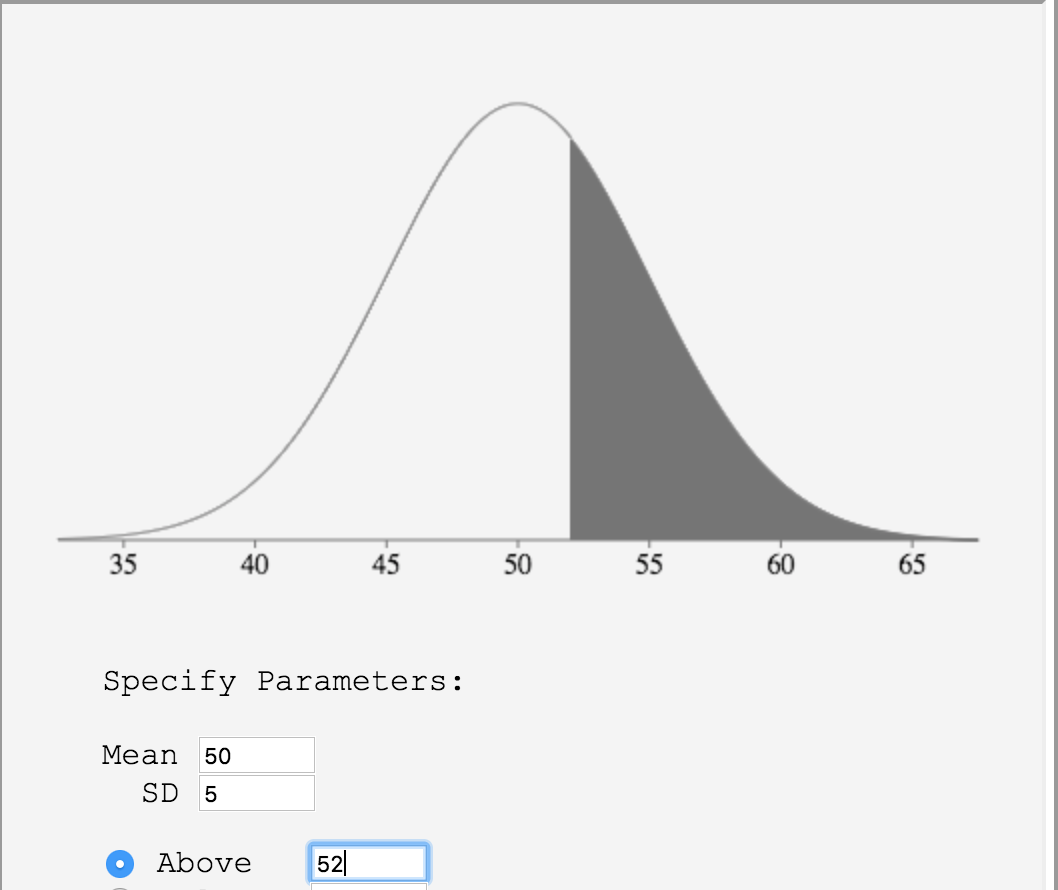
\includegraphics[width=0.5\textwidth]{figures/52.png}
    \caption{In this case the real world experiment had 52 head's tosses. Based on a normal distribution, the dark shaded area indicates the chance that you achieve 52 heads if $\hat{p_0} = 0.50$. In this case it is ~ $0.34$ }
    \label{fig:example_figure}
  \end{center}
\end{figure}

\\ 
\noindent The p-value essential tells you the probability of seeing the data that you saw in the single test trial given that you're in a boring world ($H_0$ is true). Mathematically this means $p($Data $\mid$ $H_0 =$ true).\\

\noindent
Ideally before you run the experiment you decide on a p-value threshold below which reject the hypothesis of being in a boring world. This is known as $\alpha$ or the false positive rate. Traditionally this is known to be 0.05, ie you expect to see 1 in 20 false positives. Another way to express is alpha is $\alpha = p$(reject $H_0\mid H_0 =$ true). \\

\noindent
But what about $p$(reject $H_0\mid H_0 =$ false) or the idea of power. It measures how likely is it that I reject a boring world when it is not a boring world? We want this to be high. If you want the value to big even when $H_0 false$ for small differences from boring world, ie if think boring world is false when $\hat{p_0} = 0.52$ then you need a realtively huge sample size.


\end{document}

%%% Local Variables:
%%% mode: latex
%%% TeX-master: t
%%% End:
